\documentclass[10pt,hyperref={CJKbookmarks=true},envcountsect,mathserif]{beamer}

\mode<presentation> {

% The Beamer class comes with a number of default slide themes
% which change the colors and layouts of slides. Below this is a list
% of all the themes, uncomment each in turn to see what they look like.

%\usetheme{default}
%\usetheme{AnnArbor}%不好看
\usetheme{Antibes}%block可以,但是排版不好
%\usetheme{Bergen}%目录在旁边
%\usetheme{Berkeley}%目录在旁边,同时上方有横条
%\usetheme{Berlin}
%\usetheme{Boadilla}
\usetheme{CambridgeUS}
%\usetheme{Copenhagen}%block不错,但是色调不大好
%\usetheme{Darmstadt}%%整体不错,就是下方木有横条,色调为黑紫
%\usetheme{Dresden}%%不错,和berlin类似,就是block 是个空白的
%\usetheme{Frankfurt}%和copenhagen相似
%\usetheme{Goettingen}%目录在右方,block不好
%\usetheme{Hannover}%感觉不错,目录在左方,标题在右方
%\usetheme{Ilmenau}%%很不错,和berlin类似,block也很好,但是条目风格不好,为圆形
%\usetheme{JuanLesPins}%目录在上,不是很好,block可以
%\usetheme{Luebeck}%%一般,色调不好,平直风格,配上\usecolortheme{seahorse}还不错
%\usetheme{Madrid}%%还不错,就是上方是白色的,block 也还可以
%\usetheme{Malmoe}%类似luebeck,色调不好,block不好
%\usetheme{Marburg}%目录在右方,深色调,一般
%\usetheme{Montpellier}%平直简约风格,下方木有条,不好,block也不是很好
%\usetheme{PaloAlto}%类似Berkeley,block也比较好
%\usetheme{Pittsburgh}%%%超简约风格,标题在右上角
%\usetheme{Rochester}%%简约平直风格,无上下目录横条
%\usetheme{Singapore}%%简约华丽风格
%\usetheme{Szeged}%类似berlin,但是block不好
%\usetheme{Warsaw}%浮夸复杂风格,但是色调不好

% As well as themes, the Beamer class has a number of color themes
% for any slide theme. Uncomment each of these in turn to see how it
% changes the colors of your current slide theme.

%\usecolortheme{albatross}%蓝色透明
\usecolortheme{beaver}%红色
%\usecolortheme{beetle}%灰色透明风格
%\usecolortheme{crane}%黄色
%\usecolortheme{dolphin}%蓝色
%\usecolortheme{dove}%白色
%\usecolortheme{fly}%灰色透明
%\usecolortheme{lily}%深蓝色
%\usecolortheme{orchid}%深蓝
%\usecolortheme{rose}%深蓝
%\usecolortheme{seagull}%灰白
%\usecolortheme{seahorse}%银色
%\usecolortheme{whale}%深蓝色
%\usecolortheme{wolverine}%蓝黄

%\setbeamertemplate{footline} % To remove the footer line in all slides uncomment this line
%\setbeamertemplate{footline}[page number] % To replace the footer line in all slides with a simple slide count uncomment this line

%\setbeamertemplate{navigation symbols}{} % To remove the navigation symbols from the bottom of all slides uncomment this line
}
\usepackage{graphicx} % Allows including images
\usepackage{booktabs} % Allows the use of \toprule, \midrule and \bottomrule in tables
%\usepackage{xeCJK}
%\setCJKmainfont{KaiTi}
%\usepackage{ctex}
\usepackage{bm}
\usepackage{hyperref}
\usepackage{color}
\usepackage{amsmath}
\usepackage{indentfirst}
\usepackage{fancyhdr}
\usepackage{media9}

\usepackage{amscd}
\renewcommand\familydefault{\sfdefault}
%\pgfdeclareimage[height=2cm]{logo}{logo.jpg}
%\logo{\pgfuseimage{logo}}

%----------------------------------------------------------------------------------------
%	TITLE PAGE
%----------------------------------------------------------------------------------------
\begin{document}
\setbeamertemplate{theorems}[numbered]
\newcommand{\myarray}[2]{$#1_1,#1_2,\dots,#1_#2$}

\AtBeginSection[MMLab]{
\begin{frame}
     \frametitle{Content}
   \tableofcontents[currentsection,currentsubsection,subsectionstyle =show/hide/hide]
   \end{frame}
 }



\title{Bridge the Gap between Deep RL and Human Learning}
%\subtitle{Toward Self-Awareness in Deep Reinforcement Learning}
\author[Hao SUN]{Hao SUN\inst{*}}
\institute[MMLab @CUHK]{\inst{*}Dept. Information Engineering @CUHK}



\date{\today}

\begin{frame}
\titlepage
\end{frame}

\begin{frame}
\frametitle{Content}
\tableofcontents	
\end{frame}



\section{Introduction to Deep RL}
\subsection{Learning Paradigm}
\begin{frame}
\frametitle{An Analogy of RL Learning Paradigm}	
\begin{figure}
\centering
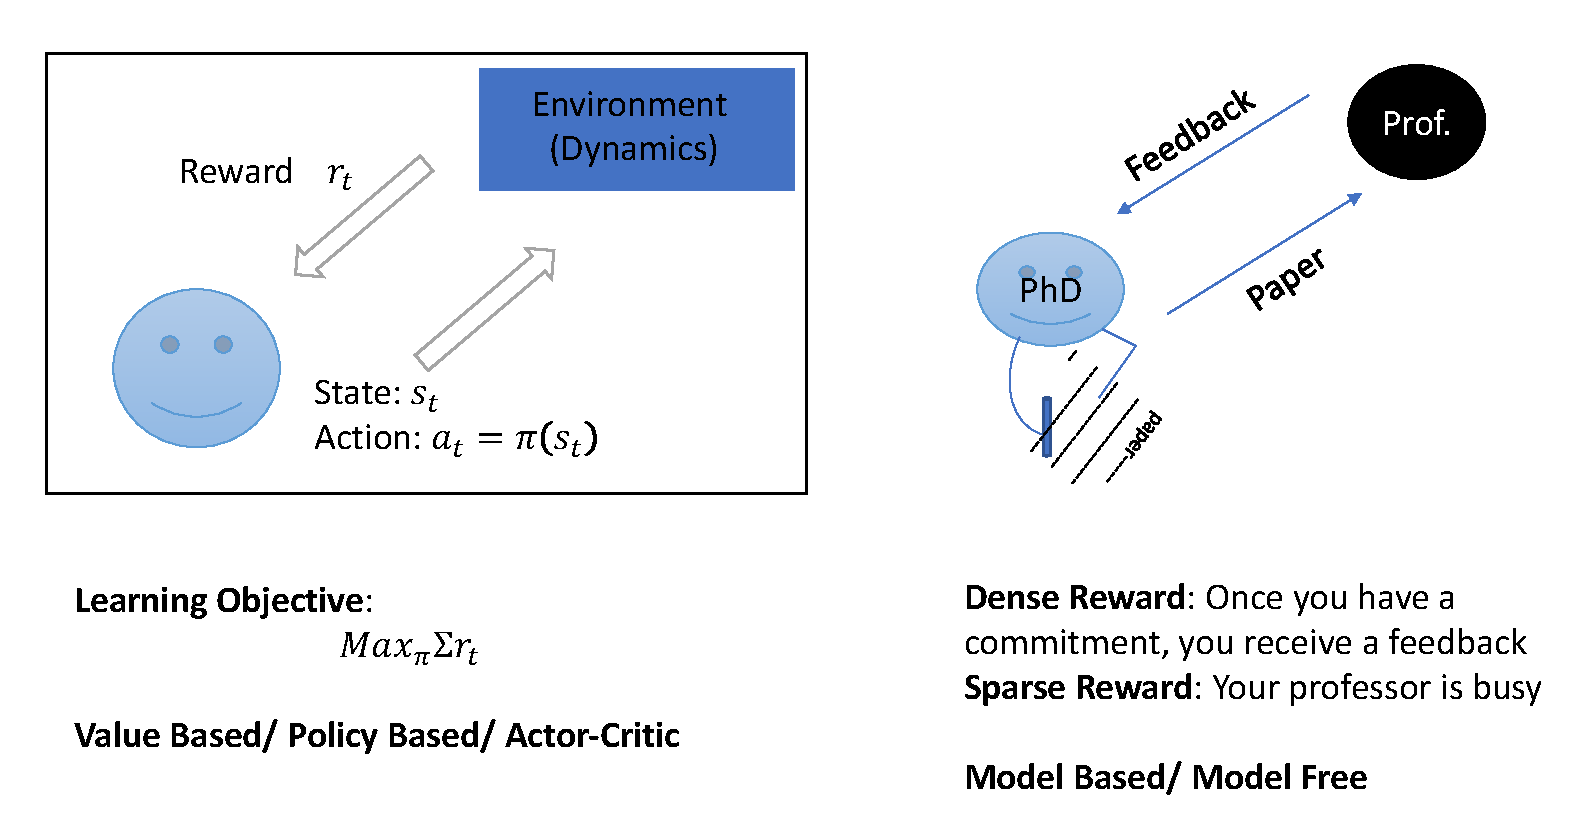
\includegraphics[width=1.0\linewidth]{figures/Prof.pdf}
\end{figure}
\end{frame}

\begin{frame}
\frametitle{Markov Decision Process (MDP) Perspective}
\begin{itemize}
	\item An agent has its policy $\pi$
	\item For each time step, the agent know about its \textbf{state} information $s_t$, it should react by giving an \textbf{action} $a_t = \pi(s_t)$, which is always a distribution over the action space $\mathcal{A}$.
	\item The \textbf{environment} (dynamics) returns a reward $r_t$
	\item Learning Objective: $\max_{\pi} \mathbb{E}_{\pi}\sum_{t=0}^T \gamma^t r_t$
	\item Markovian Property: $P(s_{t+1}|a_{t},s_{t},a_{t-1},s_{t-1},...) = P(s_{t+1}|a_{t},s_{t})$
\end{itemize}



\end{frame}


\subsection{SOTA Algorithms}
\begin{frame}
\frametitle{SOTA (Prevailing) Algorithms}
\begin{itemize}
	\item On-Policy: PPO, TRPO, A3C, A2C (Locomotion)
	\item Off-Policy: TD3, DDPG (Locomotion, HalfCheetah)
	\item Off-Policy: DQN, C51, QRDQN, IQN (Atari)
	\item Extension: Curiosity, HER (For Reward Sparse Tasks), Distributed Training
	\item Auxiliary: DQNfD, DDPGfD, Inverse RL from Human Preference
\end{itemize}


\end{frame}


\subsection{Benchmark Tasks}
\begin{frame}
\frametitle{Benchmark Tasks}	
\begin{itemize}
	\item Games (Atari, SuperMarioBros, Doom): Discrete Action Space
	\item Robotics, Locomotion based on Mujoco: Continuous Action Space
\end{itemize}
\begin{figure}
\centering
\begin{minipage}[t]{0.33\linewidth}
			\centering
			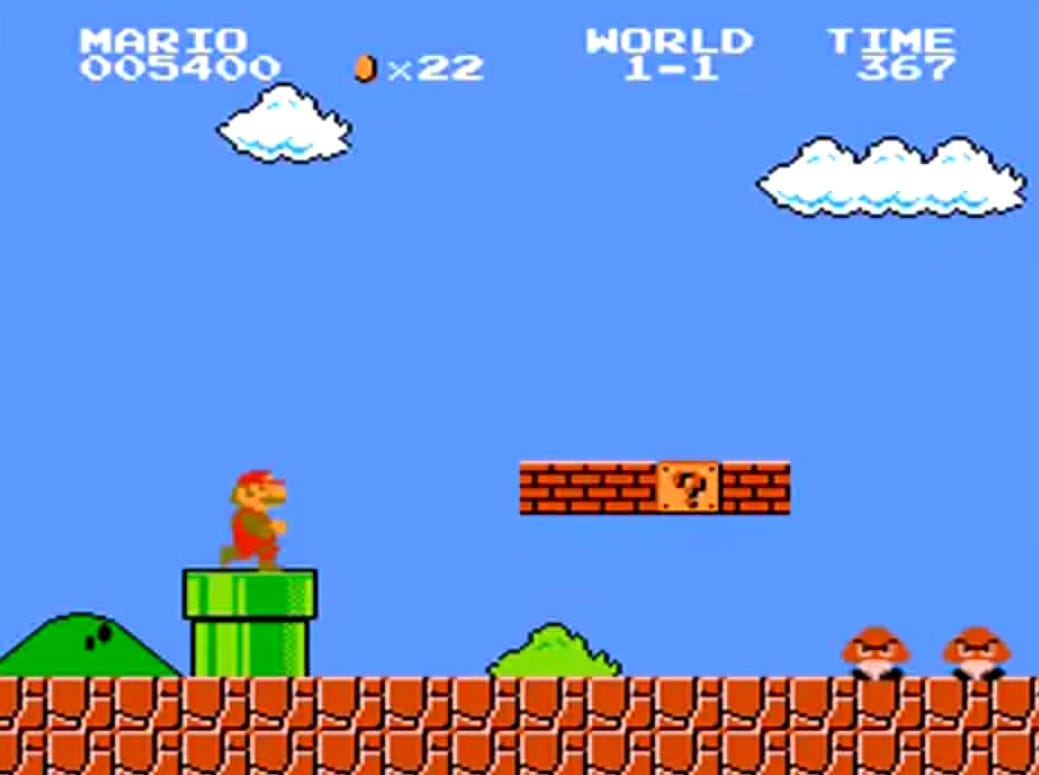
\includegraphics[width=1.3in]{figures/mariobro.jpeg}
			%\caption{1-step}
			%\label{fig:side:a}
		\end{minipage}%
		\begin{minipage}[t]{0.33\linewidth}
			\centering
			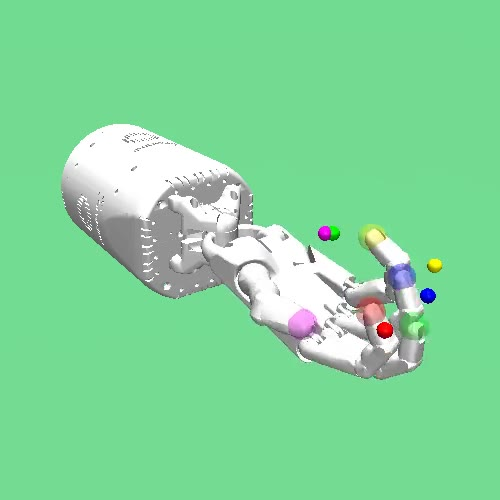
\includegraphics[width=1.0in]{figures/handreach.jpg}
			%\caption{1-step}
			%\label{fig:side:a}
		\end{minipage}%
		\begin{minipage}[t]{0.33\linewidth}
			\centering
			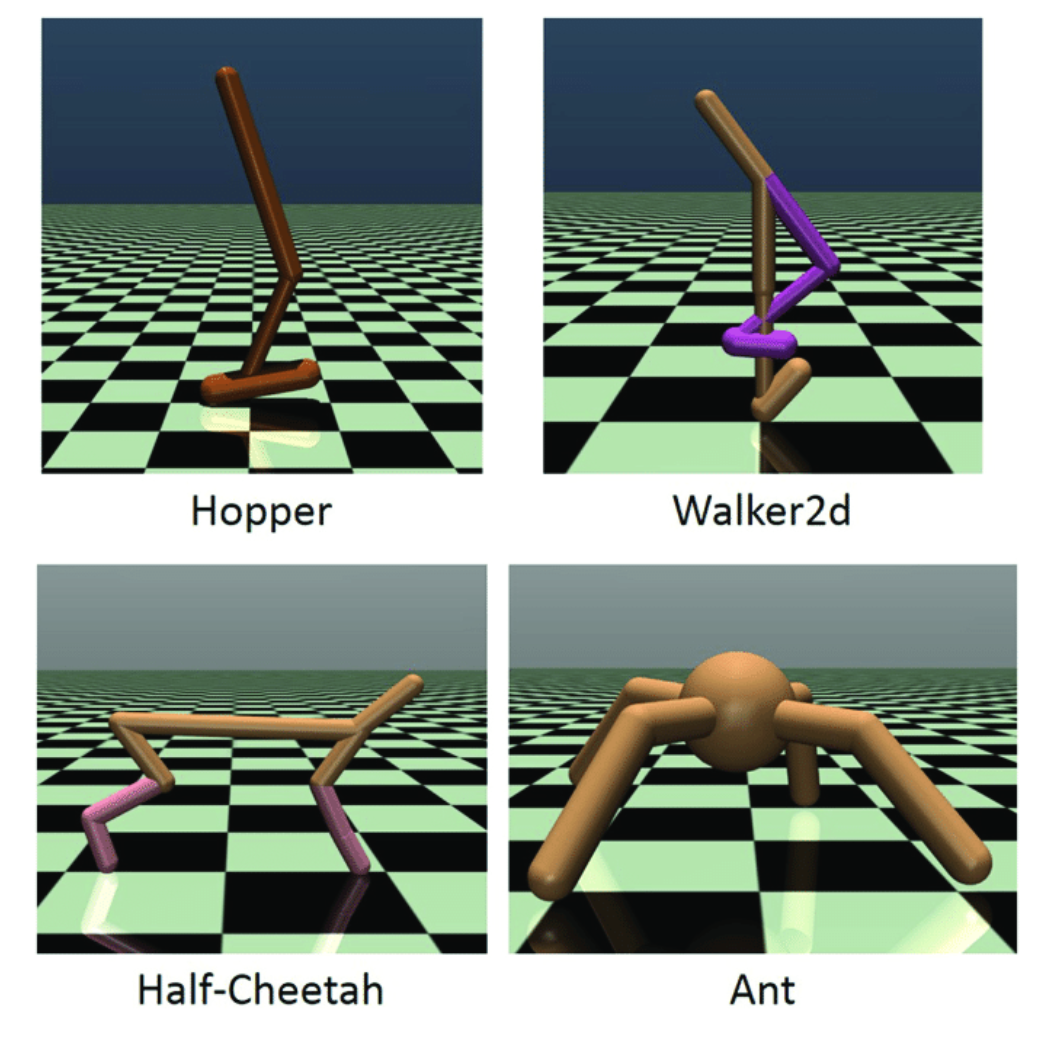
\includegraphics[width=1.0in]{figures/locomotion.png}
			%\caption{1-step}
			%\label{fig:side:a}
		\end{minipage}%
%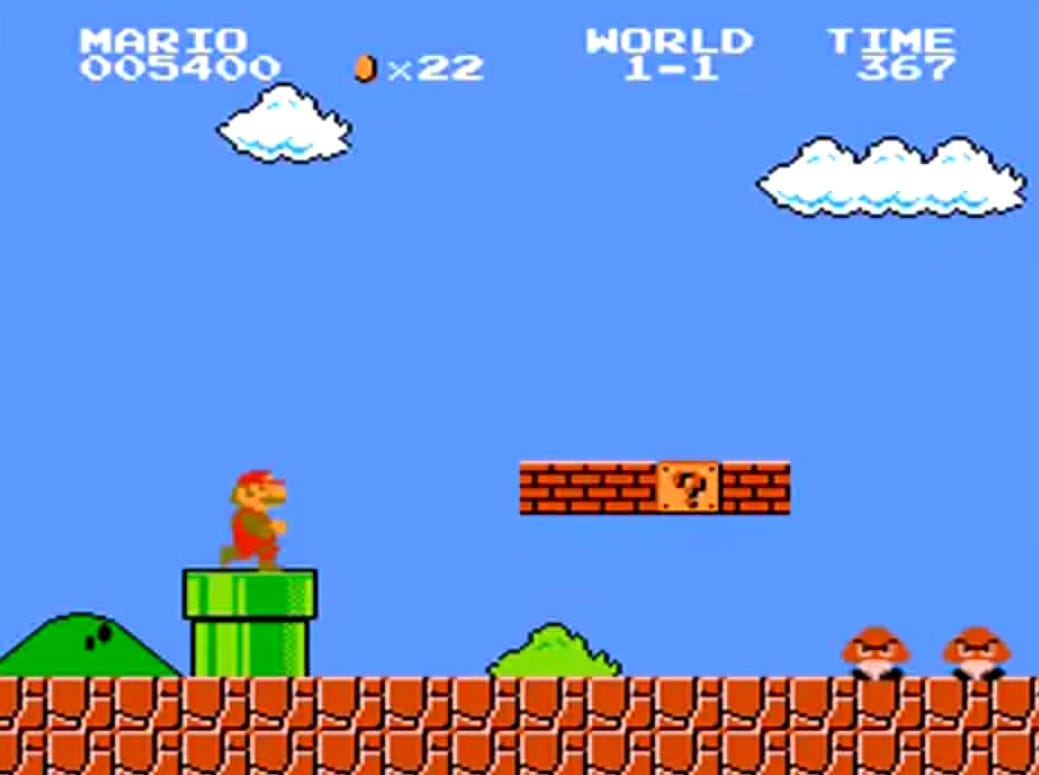
\includegraphics[width=0.3\linewidth]{figures/mariobro.jpeg}
%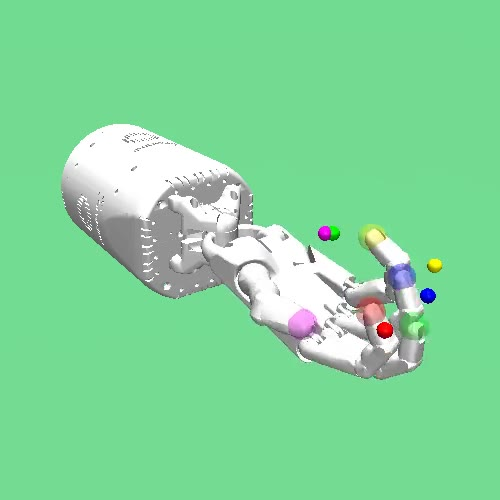
\includegraphics[width=1.07in]{figures/handreach.jpg}
%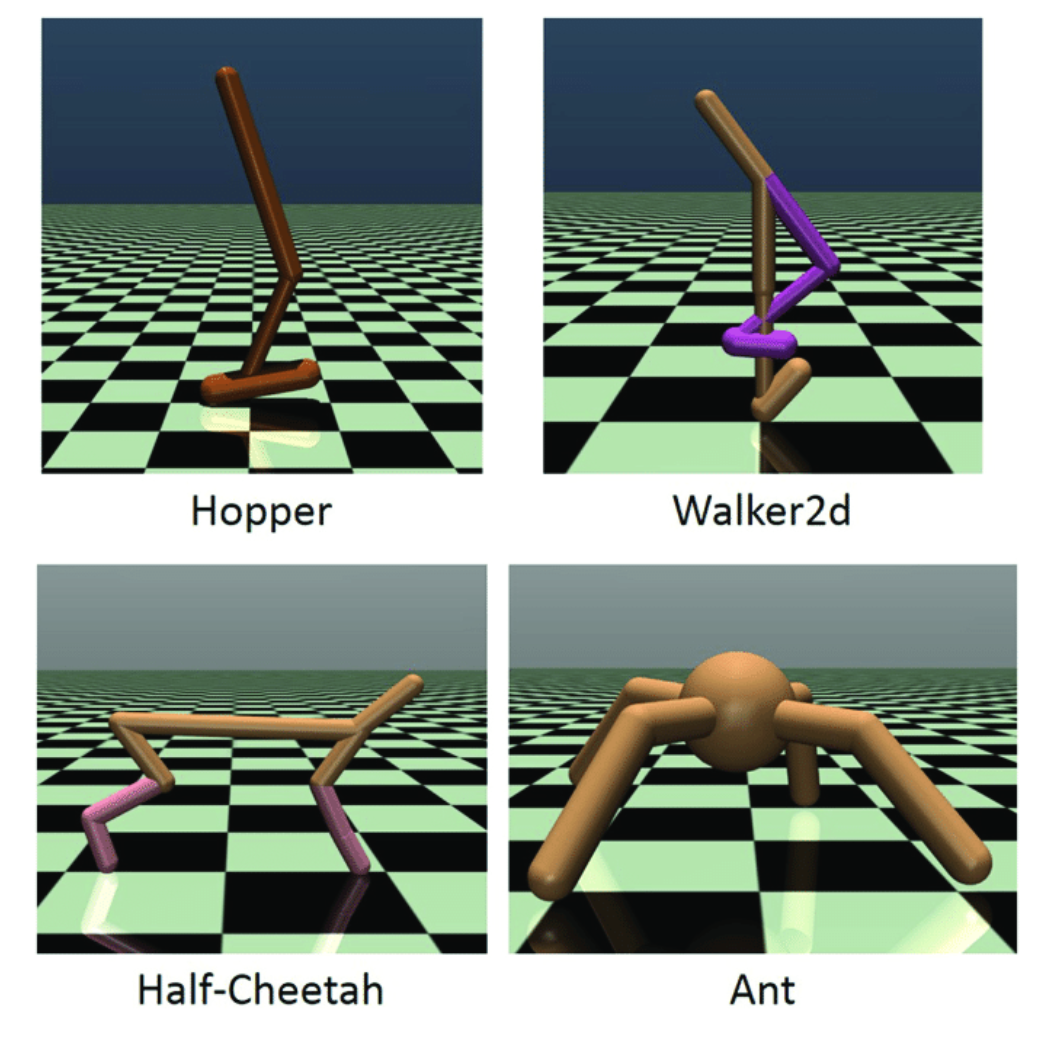
\includegraphics[width=1.1in]{figures/locomotion.png}
\caption{SuperMarioBro, HandReach and Locomotion Tasks}
\end{figure}

\end{frame}

\section{Policy Continuation with Hindsight Inverse Dynamics}
\subsection{Problem Setting}
\begin{frame}{Policy Continuation with Hindsight Inverse Dynamics}

\begin{itemize}
\item Objective: Find an effective way to learn goal-oriented reward sparse task
\item Challenge: When an agent always fail, it can hardly learn how to be success
\item Our Key Insight: Self-imitation learning of human, Curriculum learning, Learn to be success from failures
\end{itemize}
\begin{figure}
\centering
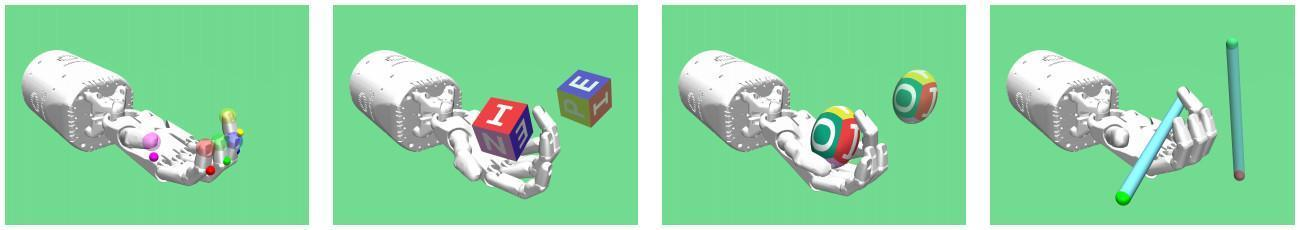
\includegraphics[width=1\linewidth]{figures/handenvs.jpeg}
%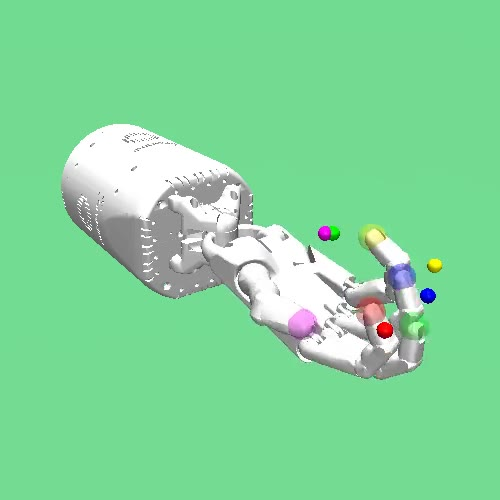
\includegraphics[width=1.07in]{figures/handreach.jpg}
%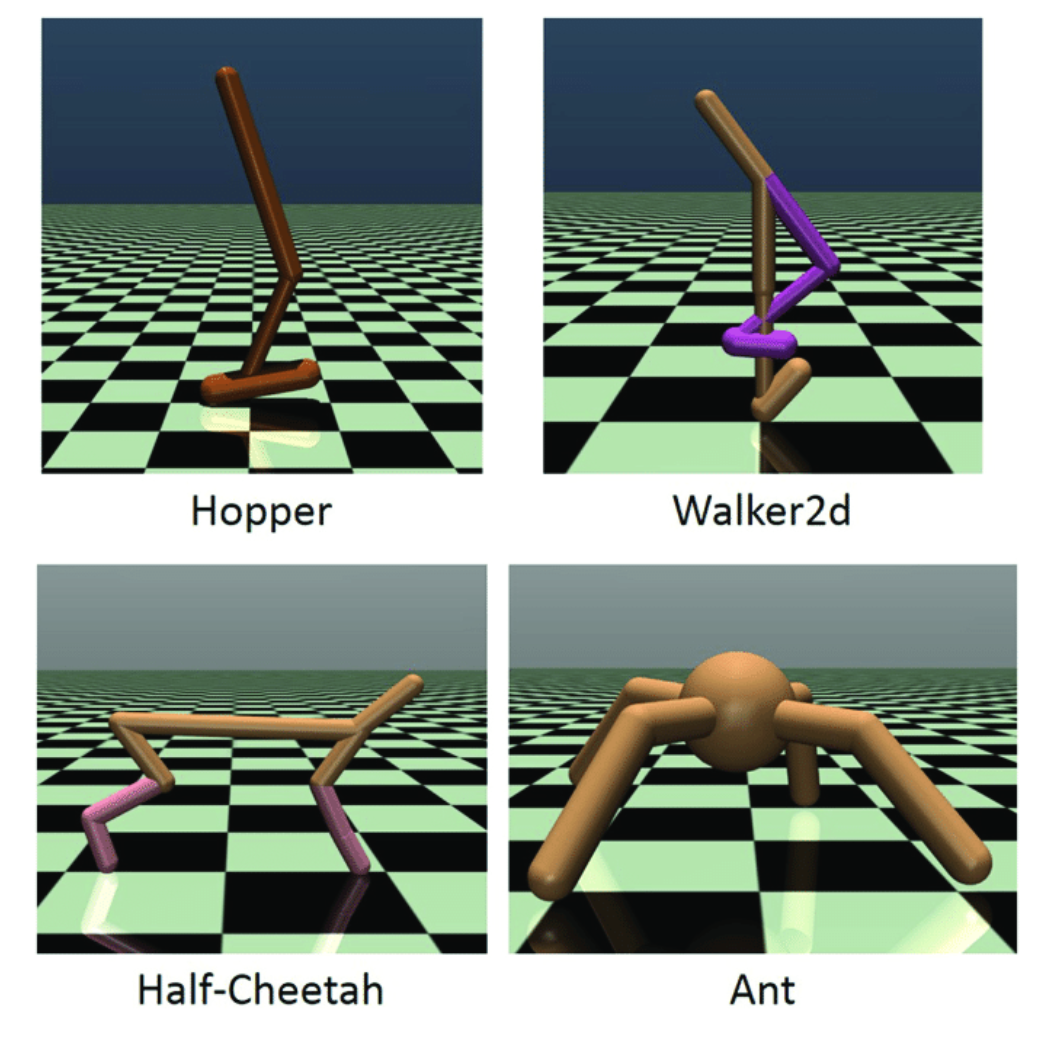
\includegraphics[width=1.1in]{figures/locomotion.png}
\caption{Hand-Reach, -Block, -Egg, -PenRotate Environment}
\end{figure}

\end{frame}

\subsection{Policy Continuation}
\begin{frame}{Policy Continuation and $k$-step Sovability}
\begin{definition}[Definition 1: Policy Continuation(PC)]%\textbf{} 
	\textit{Suppose} $\pi$ \textit{is a policy function defined on a non-empty sub-state-space} $\mathcal{S}_{U}$ \textit{of the state space} $\mathcal{S}$\textit{, i.e.,} $\mathcal{S}_{U}\subset\mathcal{S}$. \textit{If} $\mathcal{S}_{V}$ \textit{is a larger subset of} $\mathcal{S}$\textit{, containing} $\mathcal{S}_{U}$\textit{, i.e.,} $\mathcal{S}_{U}\subset\mathcal{S}_{V}$ \textit{and} $\Pi$ \textit{is a policy function defined on} $\mathcal{S}_{V}$ \textit{such that}
	$$\Pi(s) = \pi(s)\qquad \forall s\in\mathcal{S}_U $$
	\textit{then we call} $\Pi$ \textit{a policy continuation of} $\pi$\textit{, or we can say the restriction of} $\Pi$ \textit{to} $\mathcal{S}_{U}$ \textit{is the policy function} $\pi$\textit{.}
\end{definition}
\begin{itemize}
\item It is clear that complex skills are continuations of simpler skills
\end{itemize}

\begin{definition}[Definition 2: $k$-Step Solvability]
	\textit{Given a state-goal pair $(s,g)$ as a task of a certain system with deterministic dynamics, if reaching the goal $g$ needs at least $k$ steps under the optimal policy $\pi^*$ starting from $s$, i.e., starting from $s_0 = s$ and execute $a_i = \pi^*(s_i,g)$ for $i=\{0,1,...,k-1\}$, the state $s_{k} = \mathcal{T}(s_{k-1},a_{k-1})$ satisfies $m(s_k) = g$, we call the pair $(s,g)$ has $k$-step solvability, or $(s,g)$ is $k$-step solvable.}
	\end{definition}
%	Ideally the k-step solvability means the number of steps it should take from $s$ to $g$, given the maximum permitted action value. In practice the k-step solvability is a evolving concept that can gradually change during the learning process, thus is defined as "whether it can be solve with $\pi_{k-1}$ within k steps after the convergence of $\pi_{k-1}$ trained on (k-1)-step HIDs".
	
	
\end{frame}



\begin{frame}
	\frametitle{State Goal Space Partition}
\begin{definition}[Definition 3: Solvable State-Goal Space Partition]
	\textit{Given a certain environment, any solvable state-goal pairs can be categorized into only one sub state-goal space by the following partition}
	\vspace{-11pt}
	\begin{equation}
	\mathcal{S}\times\mathcal{G}\backslash(\mathcal{S}\times\mathcal{G})_{U} = \bigcup_{j=0}^T(\mathcal{S}\times\mathcal{G})_j
	\end{equation}
\end{definition}
\begin{definition}[Definition 4: Sub Policy on Sub Space]
	$\pi_i$ \textit{is a sub-policy defined on the sub-state-goal space} $(\mathcal{S}\times\mathcal{G})_i$\textit{. We say} $\pi_i^*$ \textit{is an optimal sub-policy if it is able to solve all $i$-step solvable state-goal pair tasks in $i$ steps.}
\end{definition}
	
	%Then we can progressively approximate $\pi^*$ by expanding the domain of sub-state-goal space in policy continuation from an optimal sub policy function $\pi_0^*$\footnote{In practice, such an optimal sub policy can be approximated}, i.e.,
	
	
	%and we denote the correspond optimal sub-policies as $\{\pi^*_i\}, i\in\{1,2,...,T\}$, i.e., $\{\pi^*_i\}$ can solve $i$-step solvable state-goal pairs as an optimal policy and
\begin{corollary}%[Corollary 1:]
	\label{cor1}
	\textit{If $\{\pi^*_i\}$ is restricted as a policy continuation of $\{\pi^*_{i-1}\}$ for $\forall i\in\{1,2,...k\}$, $\pi^*_i$ is able to solve any $i$-step solvable problem for $i\le k$. By definition, the optimal policy $\pi^*$ is a policy continuation of the sub policy $\pi^*_T$, and $\pi^*_T$ is already a substitute for the optimal policy $\pi^*$}.
\end{corollary}

\end{frame}

\subsection{Hindsight Inverse Dynamics}
\begin{frame}
	\frametitle{Hindsight Inverse Dynamics}
	Inverse Dynamics:
	\begin{equation}
	\label{eq_id}
	\theta_1 = \arg\min_\theta
	\sum_{s_t,g,a_t}||f_\theta((s_t,g),(s_{t+1},g))-a_t||^2
	\end{equation}


	Hindsight Inverse Dynamics:
	\begin{equation}
	\label{eq_hid}
	\theta_1 = \arg\min_\theta
	\sum_{s_t,s_{t+1},a_t}||f_\theta((s_t,m(s_{t+1})),(s_{t+1},m(s_{t+1})))-a_t||^2
	\end{equation}
		\begin{figure}[tbp]
	
		\begin{minipage}[t]{0.5\linewidth}
			\centering
			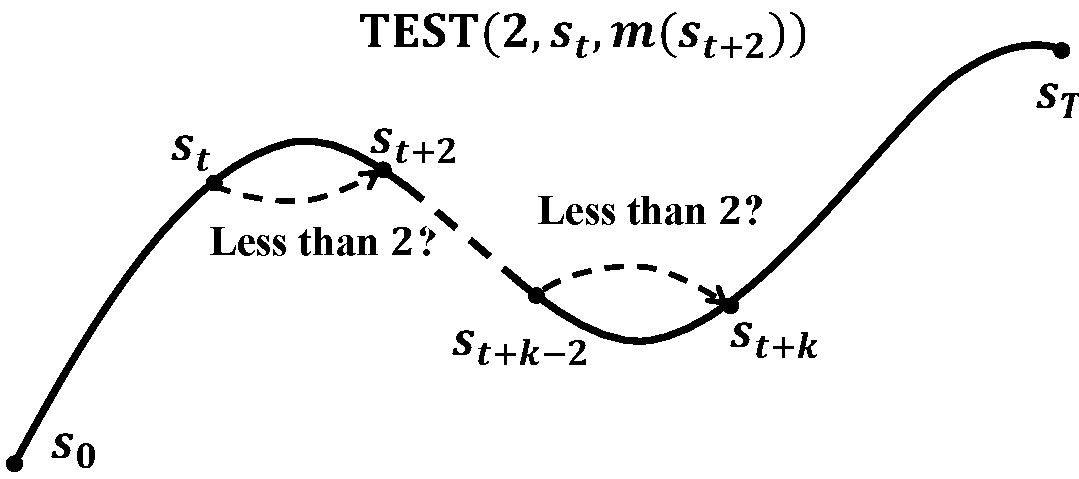
\includegraphics[width=1.9in]{figures/1step.pdf}
			%\caption{1-step}
			%\label{fig:side:a}
		\end{minipage}%
		\begin{minipage}[t]{0.5\linewidth}
			\centering
			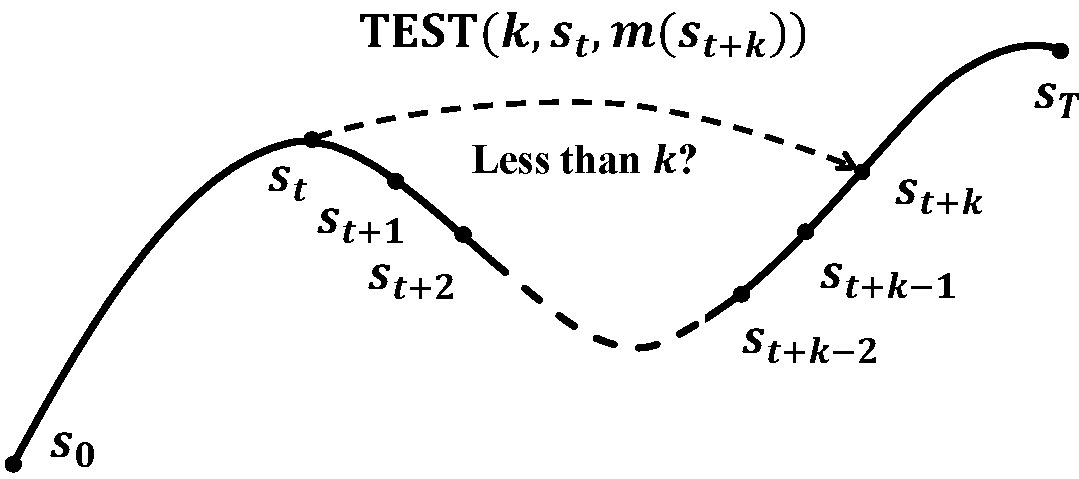
\includegraphics[width=1.9in]{figures/kstep.pdf}
			
			%\label{fig:side:b}
		\end{minipage}
		
		\caption{Test whether the transitions are 2-step (left) or $k$-step (right) solvable. The ${\rm TEST}$ function will return True if the transition $s_t\to s_{t+k}$ needs at least $k$ steps.}
		\vspace{-0.1cm}
		\label{figkstep}
	\end{figure}
	
	
\end{frame}

\subsection{Empirical Results}
\begin{frame}
	\frametitle{Empirical Results}
\begin{figure}
\centering
\begin{minipage}[t]{0.5\linewidth}
			\centering
			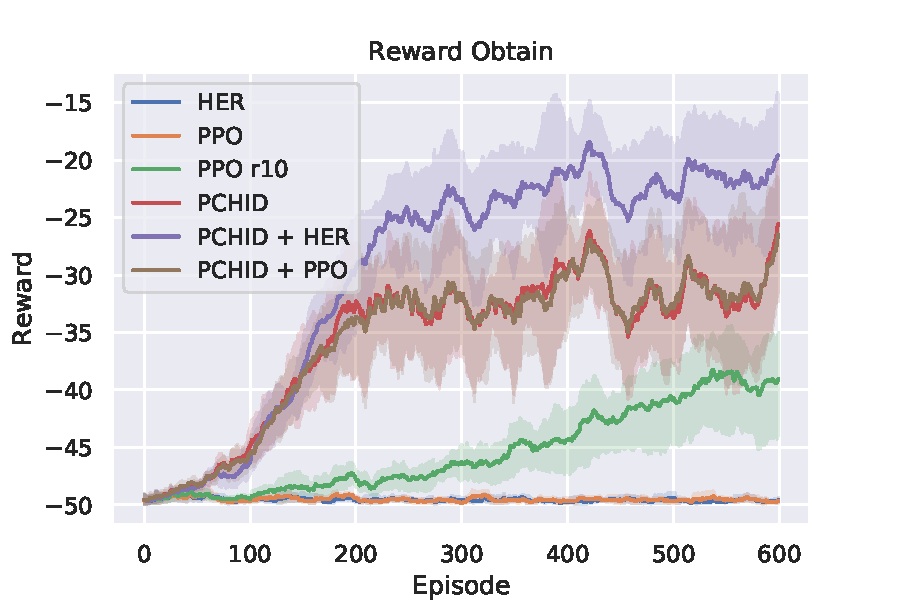
\includegraphics[width=1.6in]{figures/FR_result.pdf}
			%\caption{1-step}
			%\label{fig:side:a}
		\end{minipage}%
		\begin{minipage}[t]{0.5\linewidth}
			\centering
			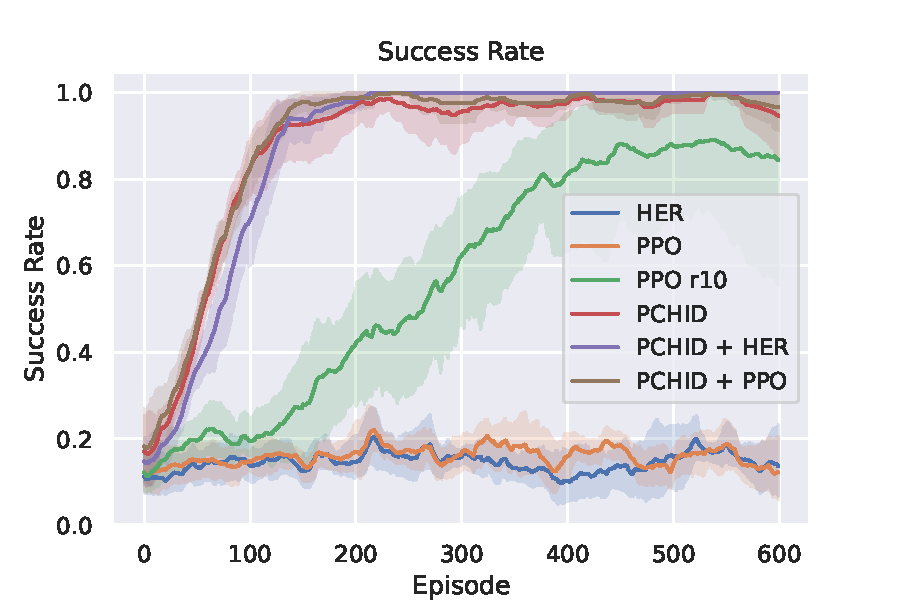
\includegraphics[width=1.6in]{figures/FR_succrate.pdf}
			%\caption{1-step}
			%\label{fig:side:a}
		\end{minipage}%

%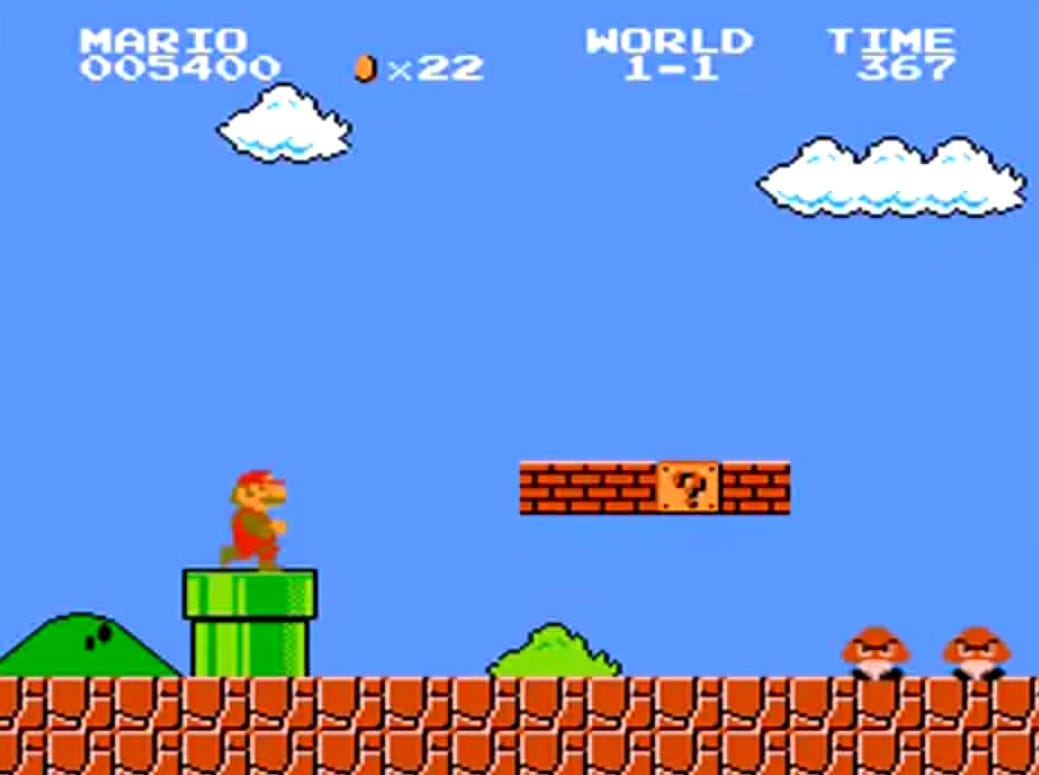
\includegraphics[width=0.3\linewidth]{figures/mariobro.jpeg}
%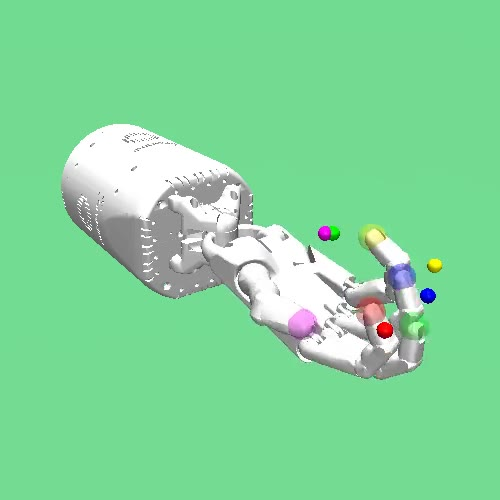
\includegraphics[width=1.07in]{figures/handreach.jpg}
%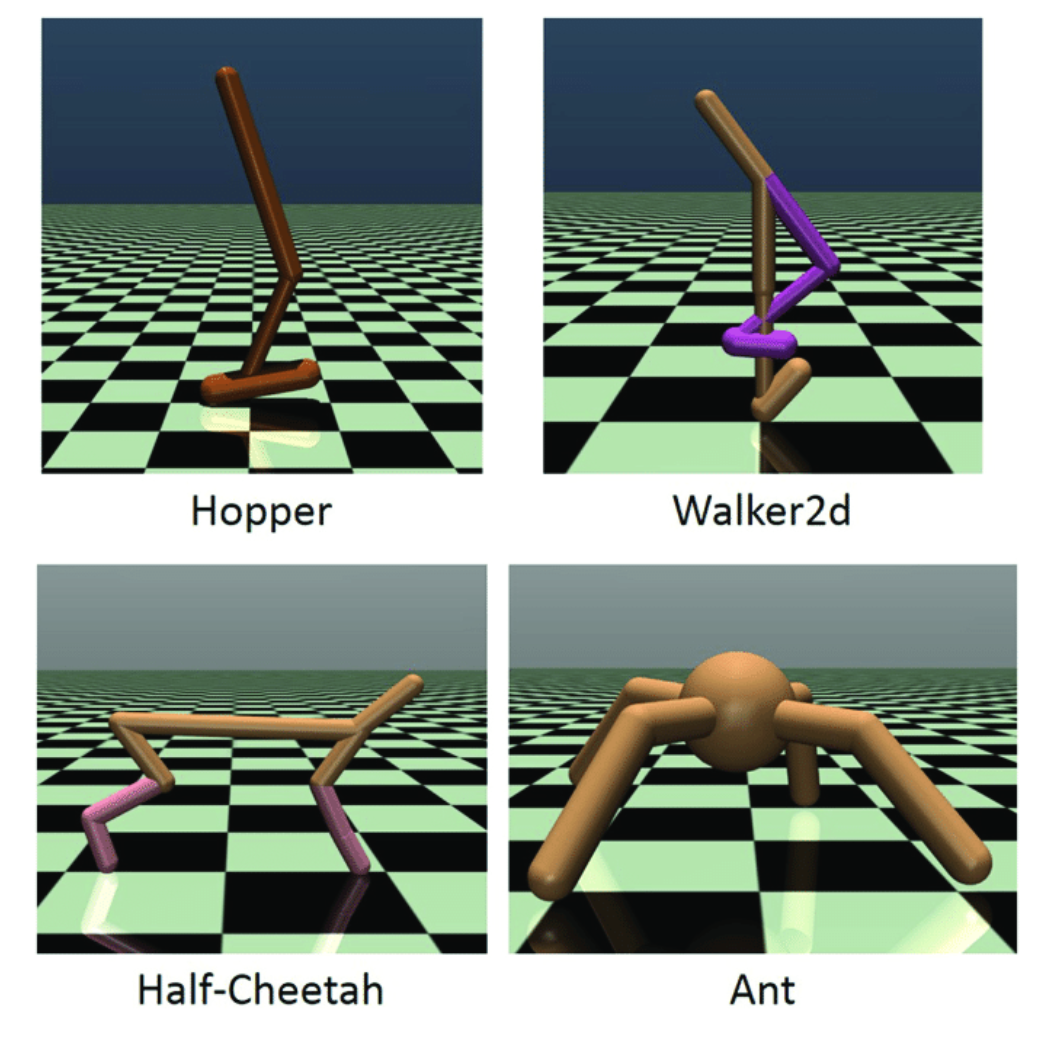
\includegraphics[width=1.1in]{figures/locomotion.png}
\caption{Experiments on the FetchReach Environment}
\end{figure}
	\begin{figure}
\centering
		\begin{minipage}[t]{0.5\linewidth}
			\centering
			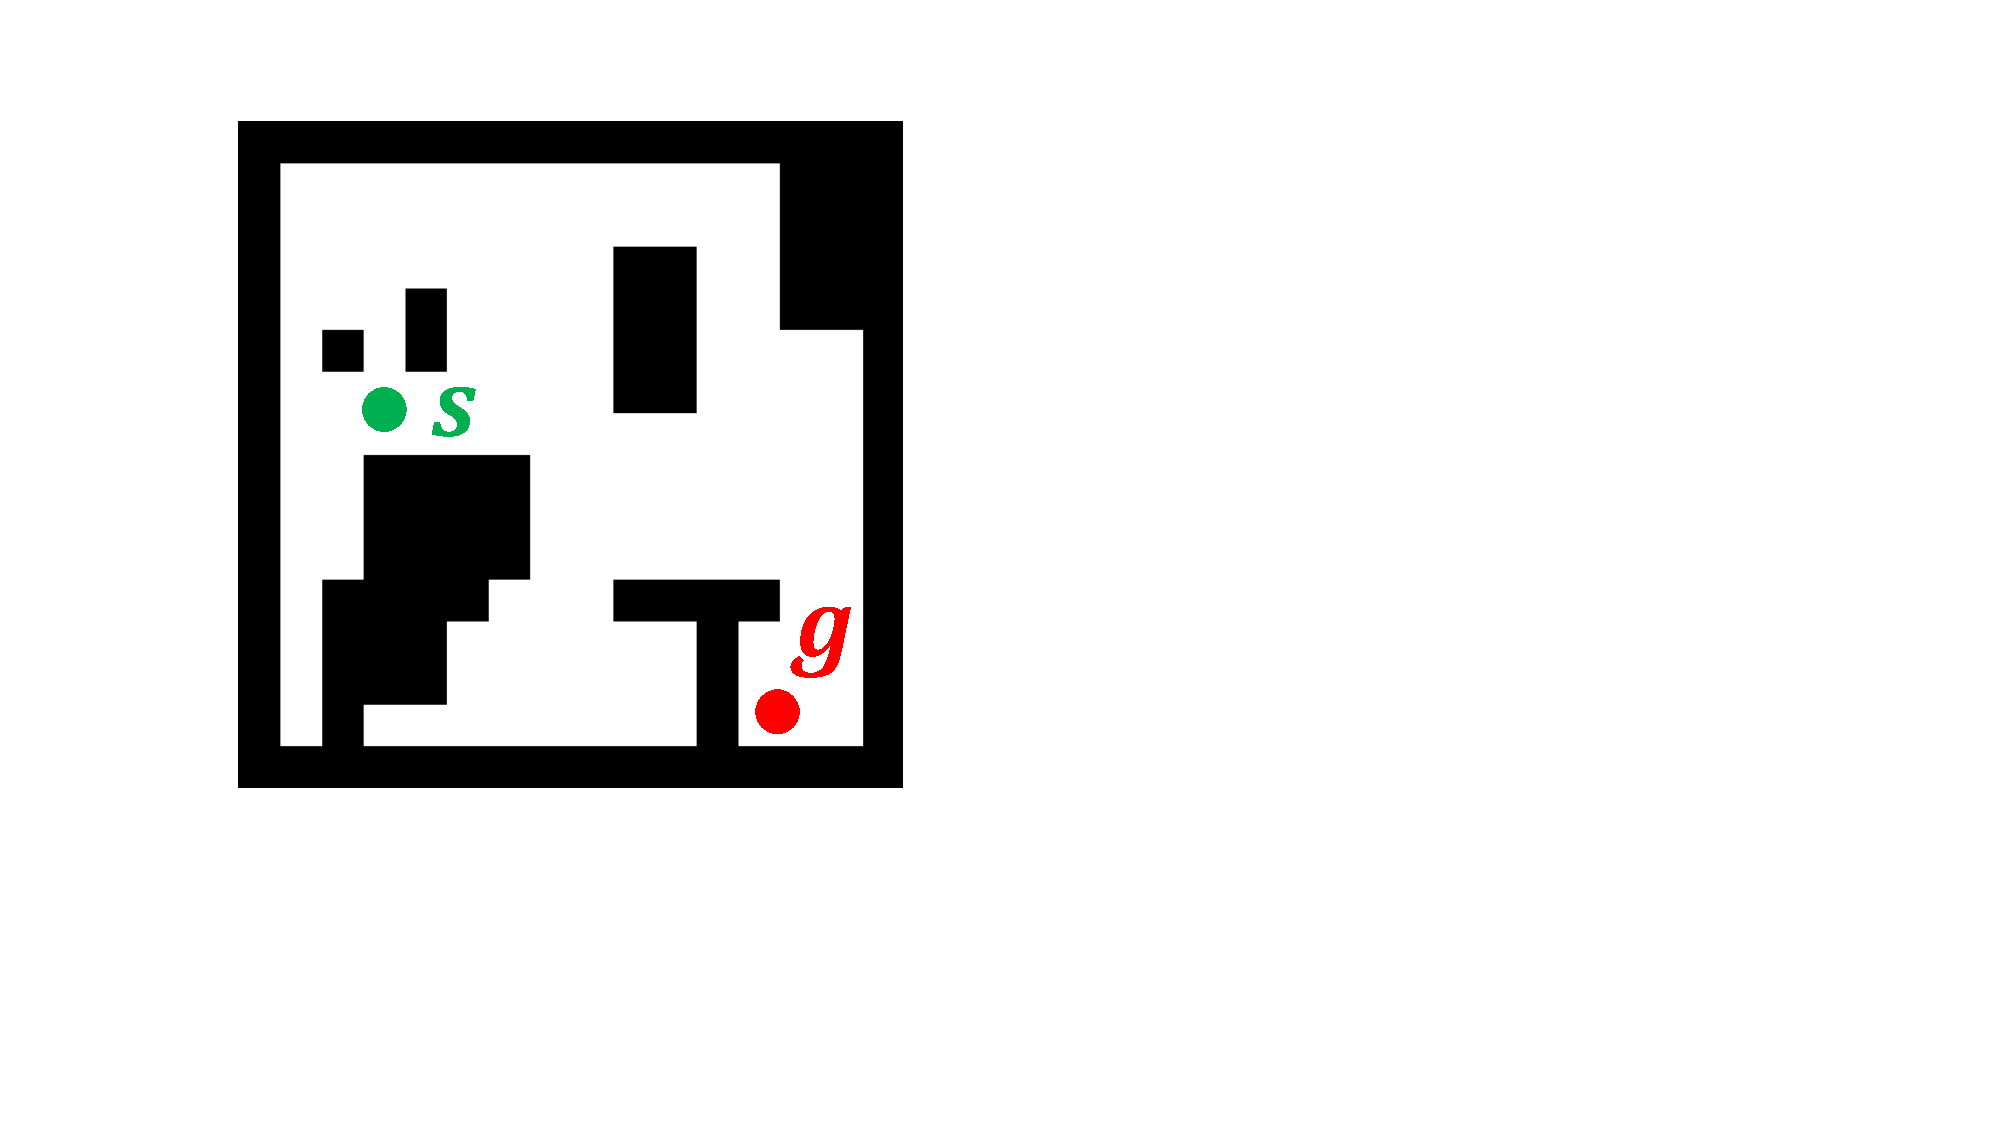
\includegraphics[width=0.9in]{figures/dm1.pdf}
			%\caption{1-step}
			%\label{fig:side:a}
		\end{minipage}%
		\begin{minipage}[t]{0.5\linewidth}
			\centering
			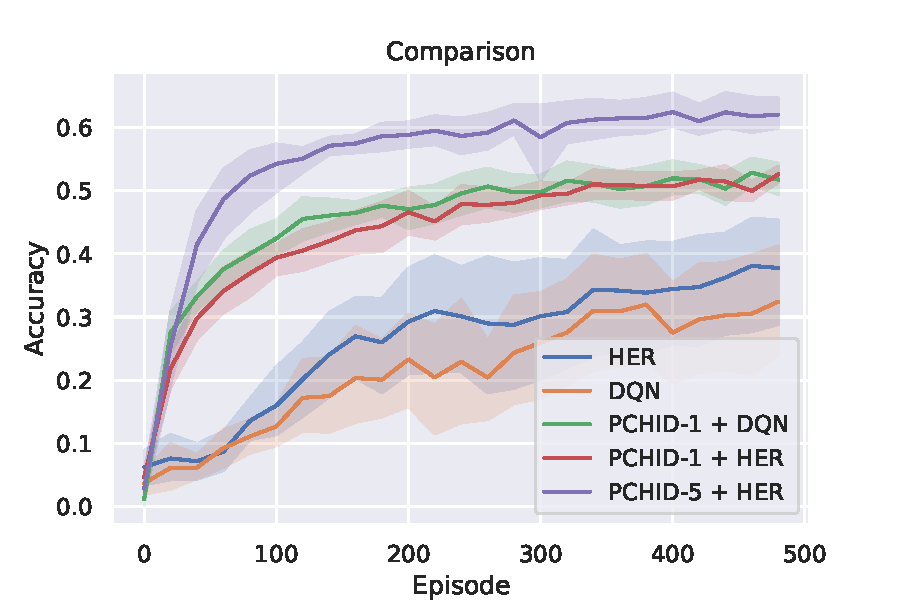
\includegraphics[width=1.6in]{figures/GW_results.pdf}
			%\caption{1-step}
			%\label{fig:side:a}
		\end{minipage}%
%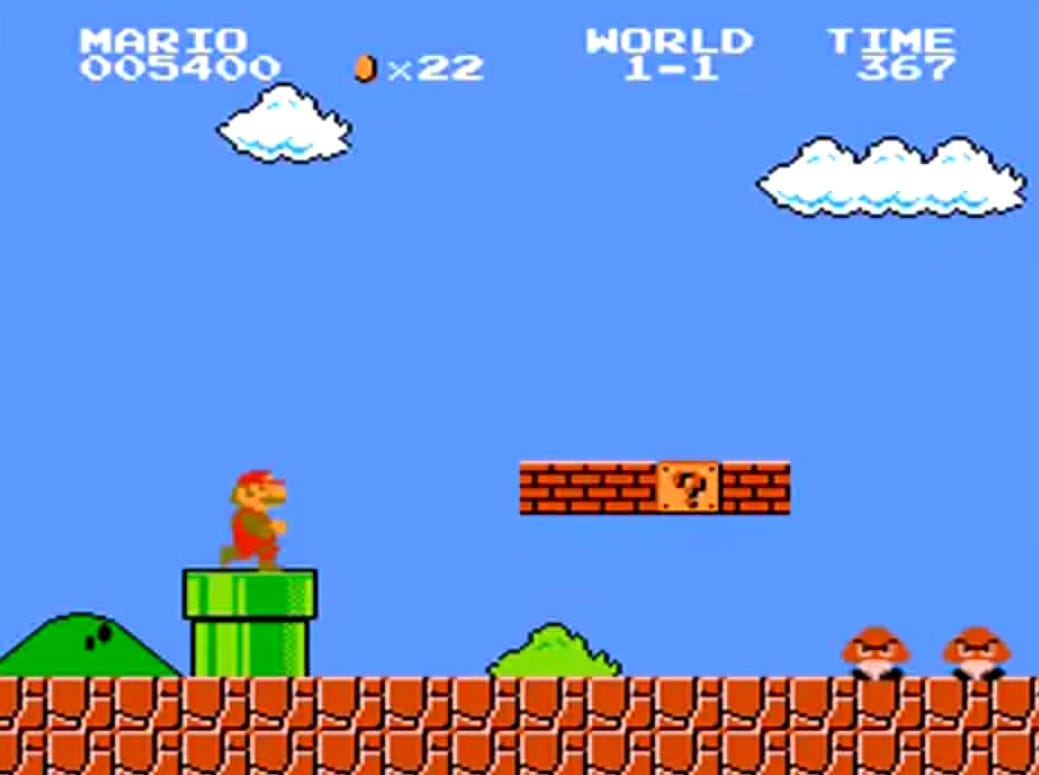
\includegraphics[width=0.3\linewidth]{figures/mariobro.jpeg}
%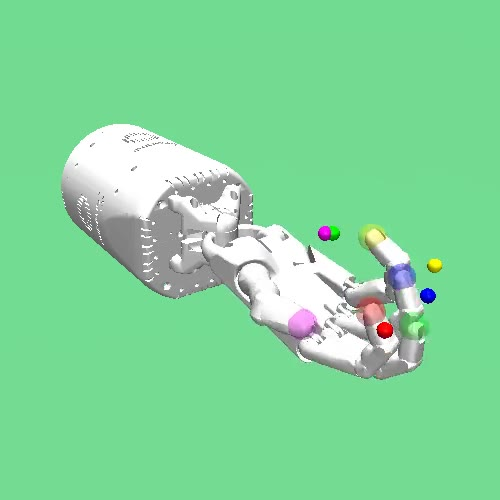
\includegraphics[width=1.07in]{figures/handreach.jpg}
%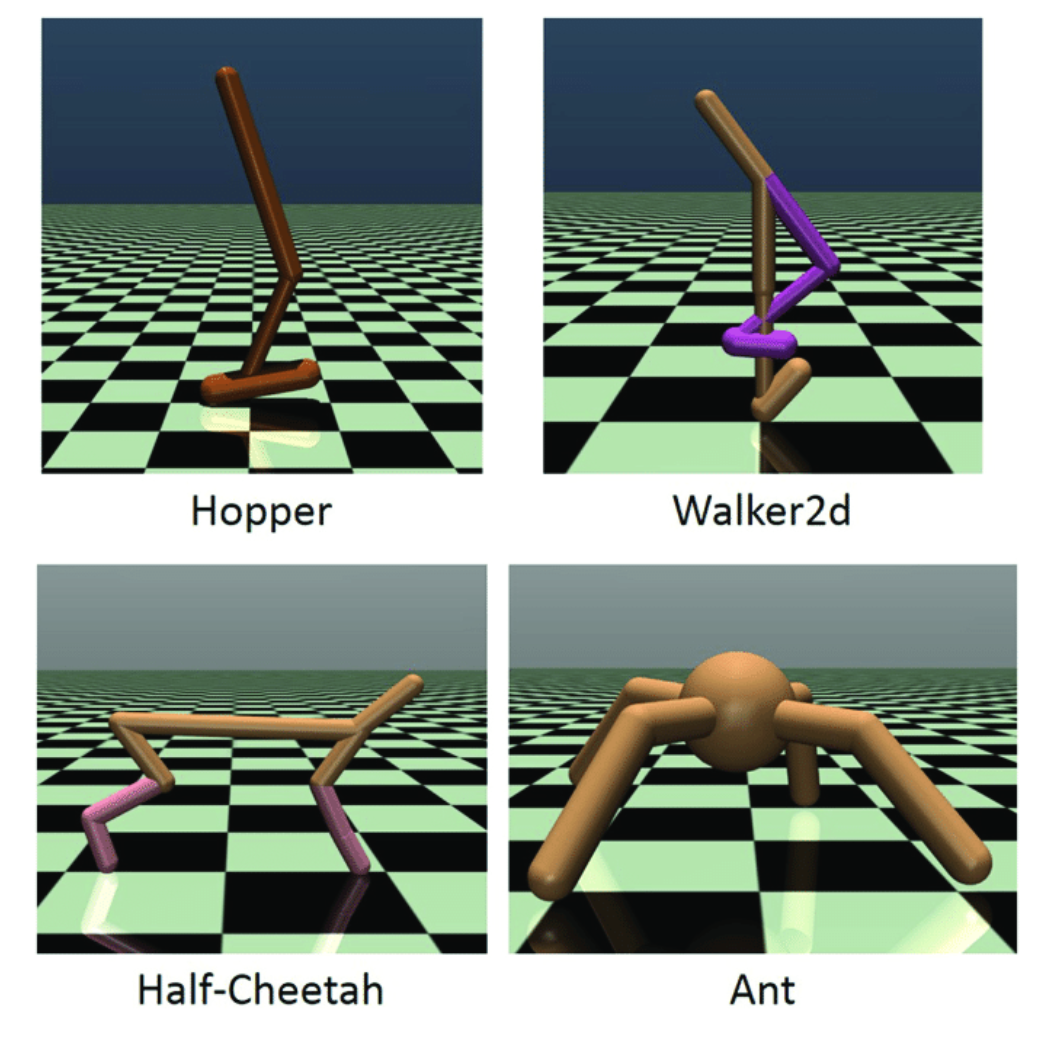
\includegraphics[width=1.1in]{figures/locomotion.png}
\caption{Experiments on the GridWorld Environment}
\end{figure}
	
\end{frame}



\section{Policy Evolution with Hindsight Inverse Dynamics}
\subsection{Introduction}

\begin{frame}{Policy Evolution with Hindsight Inverse Dynamics}

\begin{itemize}
\item Motivation: Can we further improve the learning efficiency of PCHID?
\item Question: Can we learn all the policies together? Or can the agent learn $1,2,...,k$-step transitions simultaneously?
\item Yes, from another perspective other than "Policy Continuation"
\item Why could 1-step PCHID improves the final performance? Action prediction extrapolation in \textbf{flat} state-action spaces!
\end{itemize}

\begin{figure}
\centering
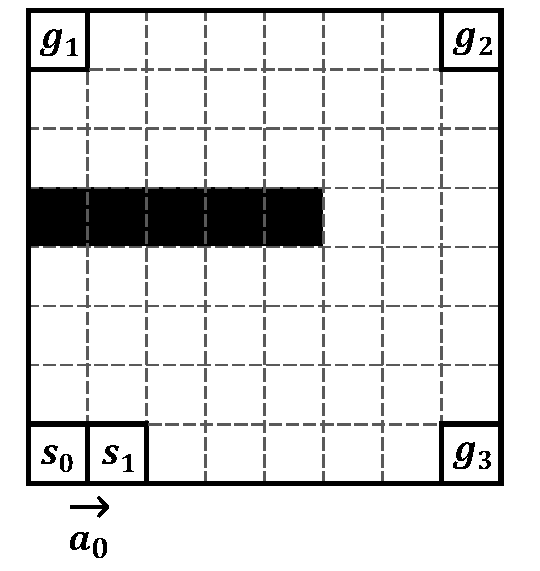
\includegraphics[width=1.1in]{figures/gridmap.pdf}
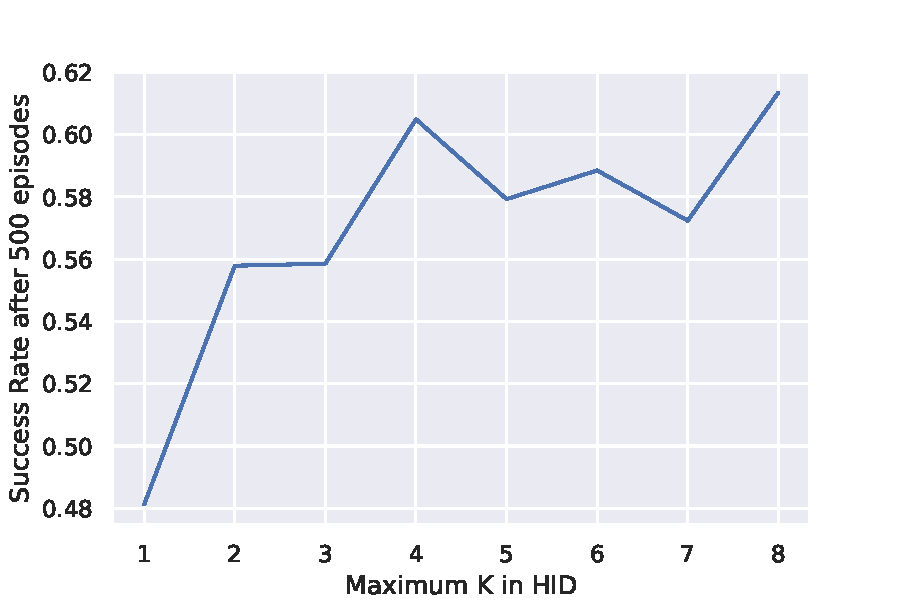
\includegraphics[width=1.9in]{figures/Max_K.pdf}
\caption{An simple navigation task; and ablation study results in the GridWorld domain}
\end{figure}
\end{frame}

%\begin{frame}
%We attribute the success of 1-step HID to the flatness of the state space, and under this circumstance extrapolation of 1-step policy works well in multistep situations. Fig.1(b) in the paper shows an analogy of how such a flatness benefits extrapolation: an agent in a grid map is asked to reach the goal $g_3$ starting from $s_0$: if the agent has already known how to reach $s_1$ in the east, intuitively, it is not difficult for it to extrapolate the policy to reach $g_3$ in the farther east. On the other hand, when the goal is at $g_1$, the barrier makes the extrapolation of 1-step policy pointing to the north fails to reach the goal. And multistep HIDs help such extrapolations in non-trivial cases. In principle, with larger K, the successful rate of extrapolation will increase. In the GridWorld environment, our ablation study (Fig.1(a) below) shows $K=4$ is able to achieve good performance. And Fig.1(b) below shows similar results in the FetchPush environment.
%
%\end{frame}

\begin{frame}
\subsection{Ornstein-Uhlenbeck Process Perspective}
	\frametitle{Ornstein-Uhlenbeck (OU) Process Perspective}
	An policy equipped with Gaussian noise in the action space $a\sim \mathcal{N}(\mu, \sigma^2)$ lead to a stochastic process in the state space. In the most simple case, the mapping between action space and the corresponding change in state space is an affine transformation, i.e., $\Delta s_t =  s_{t+1} - s_t = \alpha a_t + \beta $.
	
	Without loss of generality, we have
	\begin{equation}
		\Delta s_t \sim \mathcal{N}(\epsilon(g - s_t),\sigma^2)
	\end{equation}
	where $\epsilon$ indicates the goal awareness of the agent. e.g., for random initialized policies, the actions are unaware of goal thus $\epsilon = 0$, and for optimal policies, the actions are goal-oriented thus $\epsilon = 1$.
	So we have
	
	\begin{equation}
	\label{eq_ou}
		\mathrm{d} s_t = \epsilon (g-s_t) \mathrm{d}t + \sigma \mathrm{d}W_t
	\end{equation}
	
	Which is a typical OU process.
	
\end{frame}

\begin{frame}
	\frametitle{Intuition of Policy Evolution}
	The closed form solution of the above OU-process is 
	\begin{equation}
		s_t = s_0 e^{-\epsilon t} + g (1-e^{-\epsilon t}) + \sigma \int_0^t e^{-\epsilon(t-s)}\mathrm{d}W_s
	\end{equation}

and the expectation is
	\begin{equation}
	\label{eq_exp_ou}
		\mathbb{E}(s_t) - g = (s_0 - g )e^{-\epsilon t}
	\end{equation}
	Intuitively, Eq. (\ref{eq_exp_ou}) shows that as $\epsilon$ increase during learning, it will take less time to reach the goal. More precisely, we are caring about the concept of First Hitting Time (FHT) of OU process, i.e., $\tau = \inf\{{t>0: s_t = g|s_0 > g}\}$. 

\end{frame}

\begin{frame}
	\frametitle{Calculation of FHT}
	Without loss of generality, we can normalize the Eq.(\ref{eq_ou}) by the transformation:
	\begin{equation}
	\label{eq_transform}
		\tilde{t} = \epsilon t, \quad \tilde{s} = \frac{\sqrt{2\epsilon}}{\sigma}(s - g), \quad \tilde{g} = \frac{\sqrt{2\epsilon}}{\sigma}(g - g) = 0, \quad \tilde{s_0} = \frac{\sqrt{2\epsilon}}{\sigma}(s_0 - g)
	\end{equation}
	
	and we consider the FHT problem of 
	
	\begin{align}
	\begin{split}
		\mathrm{d} \tilde{s_t} &= - \tilde{s_t}\mathrm{d}\tilde{t} + 2\mathrm{d} W_{\tilde{t}} \\
		\tilde{\tau} &= \inf\{{\tilde{t}>0: \tilde{s_t} = 0|\tilde{s_0} > 0}\}
	\end{split}
	\end{align}
		
	The probability density function of $\tilde{\tau}$, denoted by $p_{0,\tilde{s_0}}(\tilde{t})$ is 
	
	\begin{equation}
		p_{0,\tilde{s_0}}(\tilde{t}) = \sqrt{\frac{2}{\pi}} \frac{\tilde{s_0}e^{-\tilde{t}}}{(1-e^{-2\tilde{t}})^{3/2}} \exp\left( \frac{\tilde{s_0}^2 e^{-2\tilde{t}}}{2 (1-e^{-2\tilde{t}})} \right)
	\end{equation}
	
	and the expectation is provided as %~\cite{thomas1975some,ricciardi1988first,blake1973level}
	
	\begin{equation}
	\label{eq_expectation_fht_trans}
		\mathbb{E} [\tilde{\tau}] = \sqrt{\frac{\pi}{2}} \int_{-\tilde{s_0}}^0 \left( 1 + \mathrm{erf} \left(\frac{\tilde{t}}{\sqrt{2}} \right)\right) \exp{\left(\frac{\tilde{t}^2}{2}\right)} \mathrm{d}\tilde{t}
	\end{equation}
\end{frame}

\begin{frame}
	\frametitle{Solution from FHT Perspective: Policy Evolution with HID}
	Accordingly, the optimization of solving goal-oriented reward sparse tasks can be viewed as minimizing the FHT of OU process. From this perspective, \textbf{any action that can reduce the FHT will lead to a better policy}. 

\begin{enumerate}
	\item Large $\sigma$ in exploration
	\item Large $\epsilon$ as possible
	\item Learning all transitions not yet mastered
\end{enumerate}

Here is a trade-off problem between (1) and (2), we choose to use linear decayed $\sigma$ in practice.

	\begin{table}[t]
	\caption{The successful rate of different methods in the FetchPush, FetchSlide and FetchPickAndPlace environments (trained for 1.25M timesteps)}
	\label{tab_successrate}
	\tiny
	\label{text-table}
	\centering
	\begin{tabular}{lllllll}
		\toprule & Method  & FetchPush & FetchSlide &FetchPickAndPlace    \\
		\midrule
		& PPO   & $0.00$  &   $ 0.00$&   $0.00$\\
		& DDPG   & $0.08$  &  $0.03$   &   $0.05$ \\
		& DDPG + HER   & $\bm{1.00}$  &  $0.30$   &   $0.60$ \\
		& PEHID   & $0.95$   &  $\bm{0.38}$ &   $\bm{0.75}$\\
		\bottomrule
	\end{tabular}

	\vspace{-12pt}
\end{table}
\end{frame}


\section{Learning with Social Influences}
\subsection{Introduction}

\begin{frame}{Learning with Social Influences}

\begin{itemize}
\item Motivation: Learning variant policies to solve a given primal task
\item Previous Approaches: Optimization to a \textbf{heuristically} Novelty Reward directly
\item Our Key Insight: People pursue their social uniqueness not as a goal, but a constraint.
\item Main Contributions:
\begin{enumerate}
	\item define a metric space to measure distance between policies
	\item multi-objective optimization problem $\rightarrow$ constrained optimization problem
	\item result in both different and well-performed policies
\end{enumerate}
\end{itemize}

\begin{equation}
\max_{\theta \in \Theta} \quad\mathbb{E}_{\tau \sim {\theta}} {[g_\mathrm{total}]} = 
	\max_{\theta \in \Theta} \quad \mathbb{E}_{\tau \sim {\theta}} {[\alpha \cdot g_\mathrm{task} + (1- \alpha) \cdot g_\mathrm{int}]},
\label{multiobj}
\end{equation}

\begin{equation}
\begin{split}
&\max_{\theta\in \Theta} \quad \mathbb{E}_{\tau \sim {\theta}} {[g_\mathrm{task}]}, \\
& \begin{array}{r@{\quad}r@{}l@{\quad}l}
s.t.&r_{\mathrm{int},t} - r_0 \geq 0,\forall t=1,2,...,T, \\
\end{array}
\label{constr}
\end{split}
\end{equation}

\end{frame}


\begin{frame}{Policy Metric Spaces}
\begin{theorem}[Metric Space $(\Theta,\overline{D}_{TV}^{\rho})$]
% Let $f$ be a function whose derivative exists in every point, then $f$ 
% is a continuous function.
% \end{theorem}
% \paragraph{Theorem 1}
\label{theo1} 
The expectation of $D_{TV}(\cdot,\cdot)$ of two policies over any state distribution $\rho(s)$:  % (e.g. a uniform distribution):
% \begin{align}
\begin{equation}
\overline{D}_{TV}^{\rho}({\theta_i},{\theta_j}) :={\E}_{s\sim\rho(s)}[ D_{TV}(\theta_i(s),\theta_j(s))],
% &= \sum_s\rho(s)D_{TV}(\theta_i(s),\theta_j(s))
% \end{align}
\end{equation}
is a metric on $\Theta$, thus $(\Theta,\overline{D}_{TV}^{\rho})$ is a metric space. 
\end{theorem}

\begin{definition}[Uniqueness of Policy]
Given a reference policy set $\Theta_{\text{ref}}$ such that $\Theta_{\text{ref}} = \{\theta^{ref}_i,i=1,2,...\}, \Theta_{\text{ref}}\subset\Theta$, the uniqueness $\mathrm{U}(\theta|\Theta_{\text{ref}})$ of policy $\theta$ is the minimal difference between $\theta$ and all policy in the reference policy set, i.e.,
\begin{equation}
\label{eq_unique}
    \mathrm{U}(\theta|\Theta_{\text{ref}}) := \min_{\theta_j\in \Theta_{\text{ref}}}  \overline{D}_{TV}^{\rho}(\theta,{\theta_j}).
\end{equation}
\end{definition}
\end{frame}

\subsection{Solving Constrained Optimization Problems}
\begin{frame}{Interpretation from Optimization Perspective}

\begin{theorem}[Unbiased Single Trajectory Estimation]
\label{prop_1}
The estimation of $\rho_\theta(s)$ using a single trajectory $\tau$ is unbiased.
\end{theorem}
We note here, the WSR, TNB and ours Interior Policy Differentiation (IPD) methods correspond to three approaches in constrained optimization problems. For simplicity, we consider Eq.(\ref{constr}) with a simpler constraint $g_{\mathrm{int}} - g_0 \ge 0$, where $g_{\mathrm{int}} = \sum_{t=0}^T r_{\mathrm{int},t}$, i.e.,
\begin{equation*}
\begin{split}
&\max_{\theta\in \Theta} \quad f(\theta) = \mathbb{E}_{\tau \sim {\theta}} {[g_\mathrm{task}]} \\
& \begin{array}{r@{\quad}r@{}l@{\quad}l}
s.t.&g(\theta) =g_{\mathrm{int}} - g_0 \geq 0 \\
\end{array}
\end{split}
\end{equation*}

\end{frame}



\begin{frame}{WSR: Penalty Method}
The Penalty Method considers the constraints of Eq.(\ref{constr}) by putting constraint $g(\theta)$ into a penalty term, and then solve the unconstrained problem
\begin{equation}
    \max_{\theta\in \Theta} \quad f(\theta) + \frac{1-\alpha}{\alpha}\min\{g(\theta),0\}
\end{equation}

using an iterative manner, and the limit when $\alpha \rightarrow 0$ lead to the solution of the primal constrained problem. As an approximation, WSR choose a fixed weight term $\alpha$, and use the gradient of $\nabla_{\theta}f + \frac{1-\alpha}{\alpha}\nabla_{\theta}g$ instead of $\nabla_{\theta}f + \frac{1-\alpha}{\alpha}\nabla_{\theta}\min\{g(\theta),0\}$, thus the final solution will intensely rely on the selection of $\alpha$.
\end{frame}

\begin{frame}
	\frametitle{TNB: Feasible Direction Method}

The Taylor series of $g(\theta)$ at point $\bar\theta$ is
\begin{equation}
    g(\bar\theta + \lambda \vec{p}) = g(\bar\theta) + \nabla_\theta g(\bar\theta)^{\rm{T}} \lambda \vec{p} + O(||\lambda \vec{p}||)
\end{equation}

The Feasible Direction Method (FDM) considers the constraints of Eq.(\ref{constr}) by first finding a direction $\vec{p}$ satisfies
\begin{equation}
\label{eq_10}
\begin{array}{ll}
    &\nabla_{\theta}f^{\rm{T}} \cdot \vec{p} >0 \quad \\
    &\nabla_{\theta}g^{\rm{T}} \cdot \vec{p} >0 \quad \mathrm{if}  \quad g = 0
\end{array}
\end{equation}

so that for small $\lambda$, we have
\begin{equation}
    g(\bar\theta + \lambda \vec{p}) = g(\bar\theta) + \lambda\nabla_\theta g(\bar\theta)^{\rm{T}}  \vec{p} > g(\bar\theta)=0 \quad \rm{if} \quad g(\bar\theta) = 0
\end{equation}
and 
\begin{equation}
    g(\bar\theta + \lambda \vec{p}) = g(\bar\theta) + \lambda\nabla_\theta g(\bar\theta)^{\rm{T}} \vec{p} > 0 \quad \mathrm{if} \quad g(\bar\theta) > 0
\end{equation}


\end{frame}


\begin{frame}
	\frametitle{TNB (Cont.)}
	In order to find such feasible direction $\vec{p}$, we can introduce a parameter $\eta$ in Eq.({\ref{eq_10}}), such that

\begin{equation}
\label{eq_eta}
\left\{\begin{array}{ll}
&\nabla_{\theta}f^{\rm{T}} \cdot \vec{p} >\eta  \\
&\nabla_{\theta}g^{\rm{T}} \cdot \vec{p} >\eta \quad \mathrm{if}  \quad g = 0 \\
& \eta \ge 0
\end{array}\right.
\end{equation}

As Eq.(\ref{eq_eta}) can be reformed as a linear programming (LP) problem over $\eta$, i.e.,

\begin{equation}
\label{eq_lp}
\begin{split}
&\max \eta \\
& s.t.\left\{\begin{array}{ll}
&\nabla_{\theta}f^{\rm{T}} \cdot \vec{p} >\eta  \\
&\nabla_{\theta}g^{\rm{T}} \cdot \vec{p} >\eta \quad \mathrm{if}  \quad g = 0 \\
& -1\le d_j \le 1, j=1,2,...,n
\end{array}\right.
\end{split}
\end{equation}
where $\vec{p} = (d_1,d_2,...,d_n)^\mathrm{T}$, and the last constraint prevent $|\vec{p}|$ from going to $\rightarrow \infty$ (as we only care about $\vec{p}$ as a direction). Denote the optimal solution of Eq.(\ref{eq_lp}) as $(\eta^*,\vec{p}^*)$. We can then step to the direction of $\vec{p}$ after a line search for the optimal stride $\lambda^*$. The Topkis-Veinott method provides improves FDM by using another auxiliary problem.

\end{frame}


\begin{frame}
	\frametitle{TNB (Cont.)}
	The TNB method, by using the bisector of gradients $\nabla_{\theta}f$ and $\nabla_{\theta}g$, select $\vec{p}$ to be 

\begin{equation}
\label{eq_tnb_p}
\vec{p}=\left\{\begin{array}{ll}
 \nabla_{\theta}f + \frac{|\nabla_{\theta}f|}{|\nabla_{\theta}g|} \nabla_{\theta}g \cdot \cos{(\nabla_{\theta}f,\nabla_{\theta}g)} & {\mathrm if}  \, \cos{(\nabla_{\theta}f,\nabla_{\theta}g)} \le 0\\
 \nabla_{\theta}f + \frac{|\nabla_{\theta}f|}{|\nabla_{\theta}g|} \nabla_{\theta}g &{\mathrm if}  \,
 \cos{(\nabla_{\theta}f,\nabla_{\theta}g)} > 0
\end{array}\right.
\end{equation}

Clearly, Eq.(\ref{eq_tnb_p}) satisfies Eq.(\ref{eq_10}). As the stride of TNB is chosen as $\frac{|\nabla_{\theta}f| + |\nabla_{\theta}g|}{2}$, and the $\nabla_{\theta}g$ term always exists during optimization, problem arises when $\nabla_{\theta}f\rightarrow0$, therefore the final optimization result will heavily rely on the selection of $g$. i.e., the shape of $g$ is crucial for the success of TNB.


\end{frame}
%\section{Future Directions}

\begin{frame}
	\frametitle{Interior Policy Differentiation (IPD): Interior Method}
	in this work we propose to solve the constrained optimization problem Eq.(\ref{constr}) by resembling the Interior Point Methods (IPMs). %Regarding our optimization is over possible policies $\theta$, we name our approach as Interior Policy Differentiation (IPD). \bz{The previous sentence is not clear to me}
In vanilla IPMs, the constrained optimization problem in Eq.(\ref{constr}) is solved by reforming it to an unconstrained form with an additional barrier term in the objective as
\begin{equation}
\label{eq_IPM}
    \max_{\theta\in \Theta} \quad \mathbb{E}_{\tau \sim {\theta}}[g_\mathrm{task} + \sum_{t=0}^{T}\alpha\log{(r_{\mathrm{int},t} - r_0)}].
\end{equation}
The limit of Eq.(\ref{eq_IPM}) when $\alpha\rightarrow0$ then leads to the solution of Eq.(\ref{constr}). 

However, directly applying this solution is computationally challenging and numerically unstable, especially when $\alpha$ is small. 

A more natural way can be used: since the learning process is based on sampled transitions, we can simply bound the collected transitions in the feasible region by permitting previous trained $M$ policies $\theta_i \in \Theta_{\text{ref}}, i=1,2,...,M$ sending termination signals during the training process of new agents. 

In other words, we implicitly bound the feasible region by terminating any new agent that steps outside it.
\end{frame}

\subsection{Empirical Results}
\begin{frame}
	\frametitle{Empirical Results}
	\begin{figure}[t]
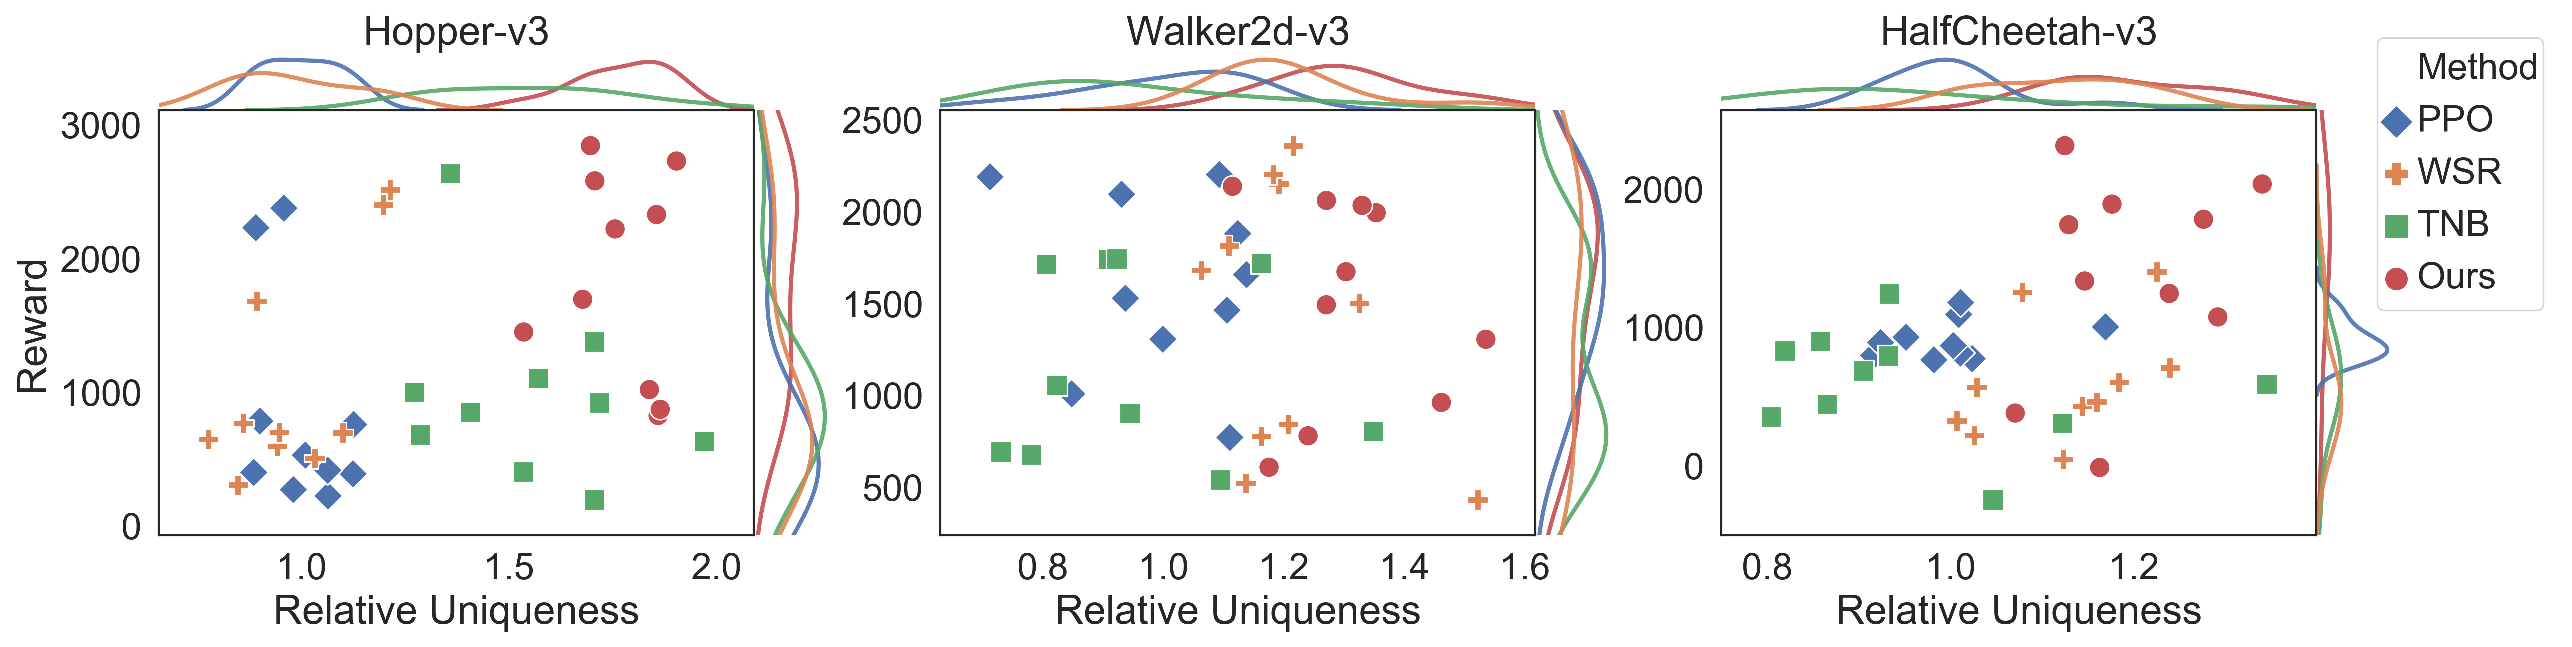
\includegraphics[width=\linewidth]{figures/v8.pdf}
% \begin{minipage}[htbp]{0.33\linewidth}
% 			\centering
%  			\includegraphics[width=1.75in]{figures/hopper_scat.pdf}
% % 			\includegraphics[width=\linewidth]{figures/fig2-pengzh/v3-1.png}
% 		\end{minipage}%
% 		\begin{minipage}[htbp]{0.33\linewidth}
% 			\centering
%  			\includegraphics[width=1.75in]{figures/walker_scat.pdf}
% % 			\includegraphics[width=\linewidth]{figures/fig2-pengzh/v3-2.png}
% 		\end{minipage}
% 		\begin{minipage}[htbp]{0.33\linewidth}
% 			\centering
%  			\includegraphics[width=1.75in]{figures/cheetah_scat.pdf} 
% %			\includegraphics[width=\linewidth]{figures/fig2-pengzh/v3-3.png}
% 		\end{minipage}
\caption{The comparison between Uniqueness and Performance in Hopper-v3, Walker2d-v3 and HalfCheetah-v3 environments. The value of uniqueness is normalized to relative uniqueness by regarding the averaged uniqueness of PPO policies as the baseline.}
%{\color{red} 1. ok now our main results are from PS [doge] (fixed fig.3 a)}

%\pengzh{Response: 3. the hopper has exactly same curve between PPO and WSR so it's coved by the yellow line.}

\label{fig_novelty}
\end{figure}
\end{frame}

\begin{frame}{Accepted Works}

\begin{itemize}
\item Policy Continuation with Hindsight Inverse Dynamics (NeurIPS'19)
\item Policy Continuation and Policy Evolution with Hindsight Inverse Dynamics (NeurIPS'19 OptRL Workshop)
\item Learning with Identity and Uniqueness through Social Constraints (NeurIPS'19 DeepRL Workshop)
\end{itemize}
%\pause
\huge{\centerline{Thanks!}}
\end{frame}














\end{document}
